\chapter{ТЕСТИРОВАНИЕ СИСТЕМЫ УПРАВЛЕНИЯ РОБОТОМ-ГЕКСАПОДОМ}

В данной главе приводится тестирование решения полученного в ходе выпускной бакалаврской работы.

Для полной проверки работоспособности реализованной системы управления роботом-гексподом необходимо:

\begin{itemize}
	\item Протестировать адаптивность и кросплатформенность web интерфейса;
	\item Протестировать синхронизацию параметров между разными экземплярами интерфейса;
	\item Различные походки, путем управления как с web интерфейса, так и с аппаратного джойстика.
\end{itemize}

\begin{figure}[h!]
	\centering
	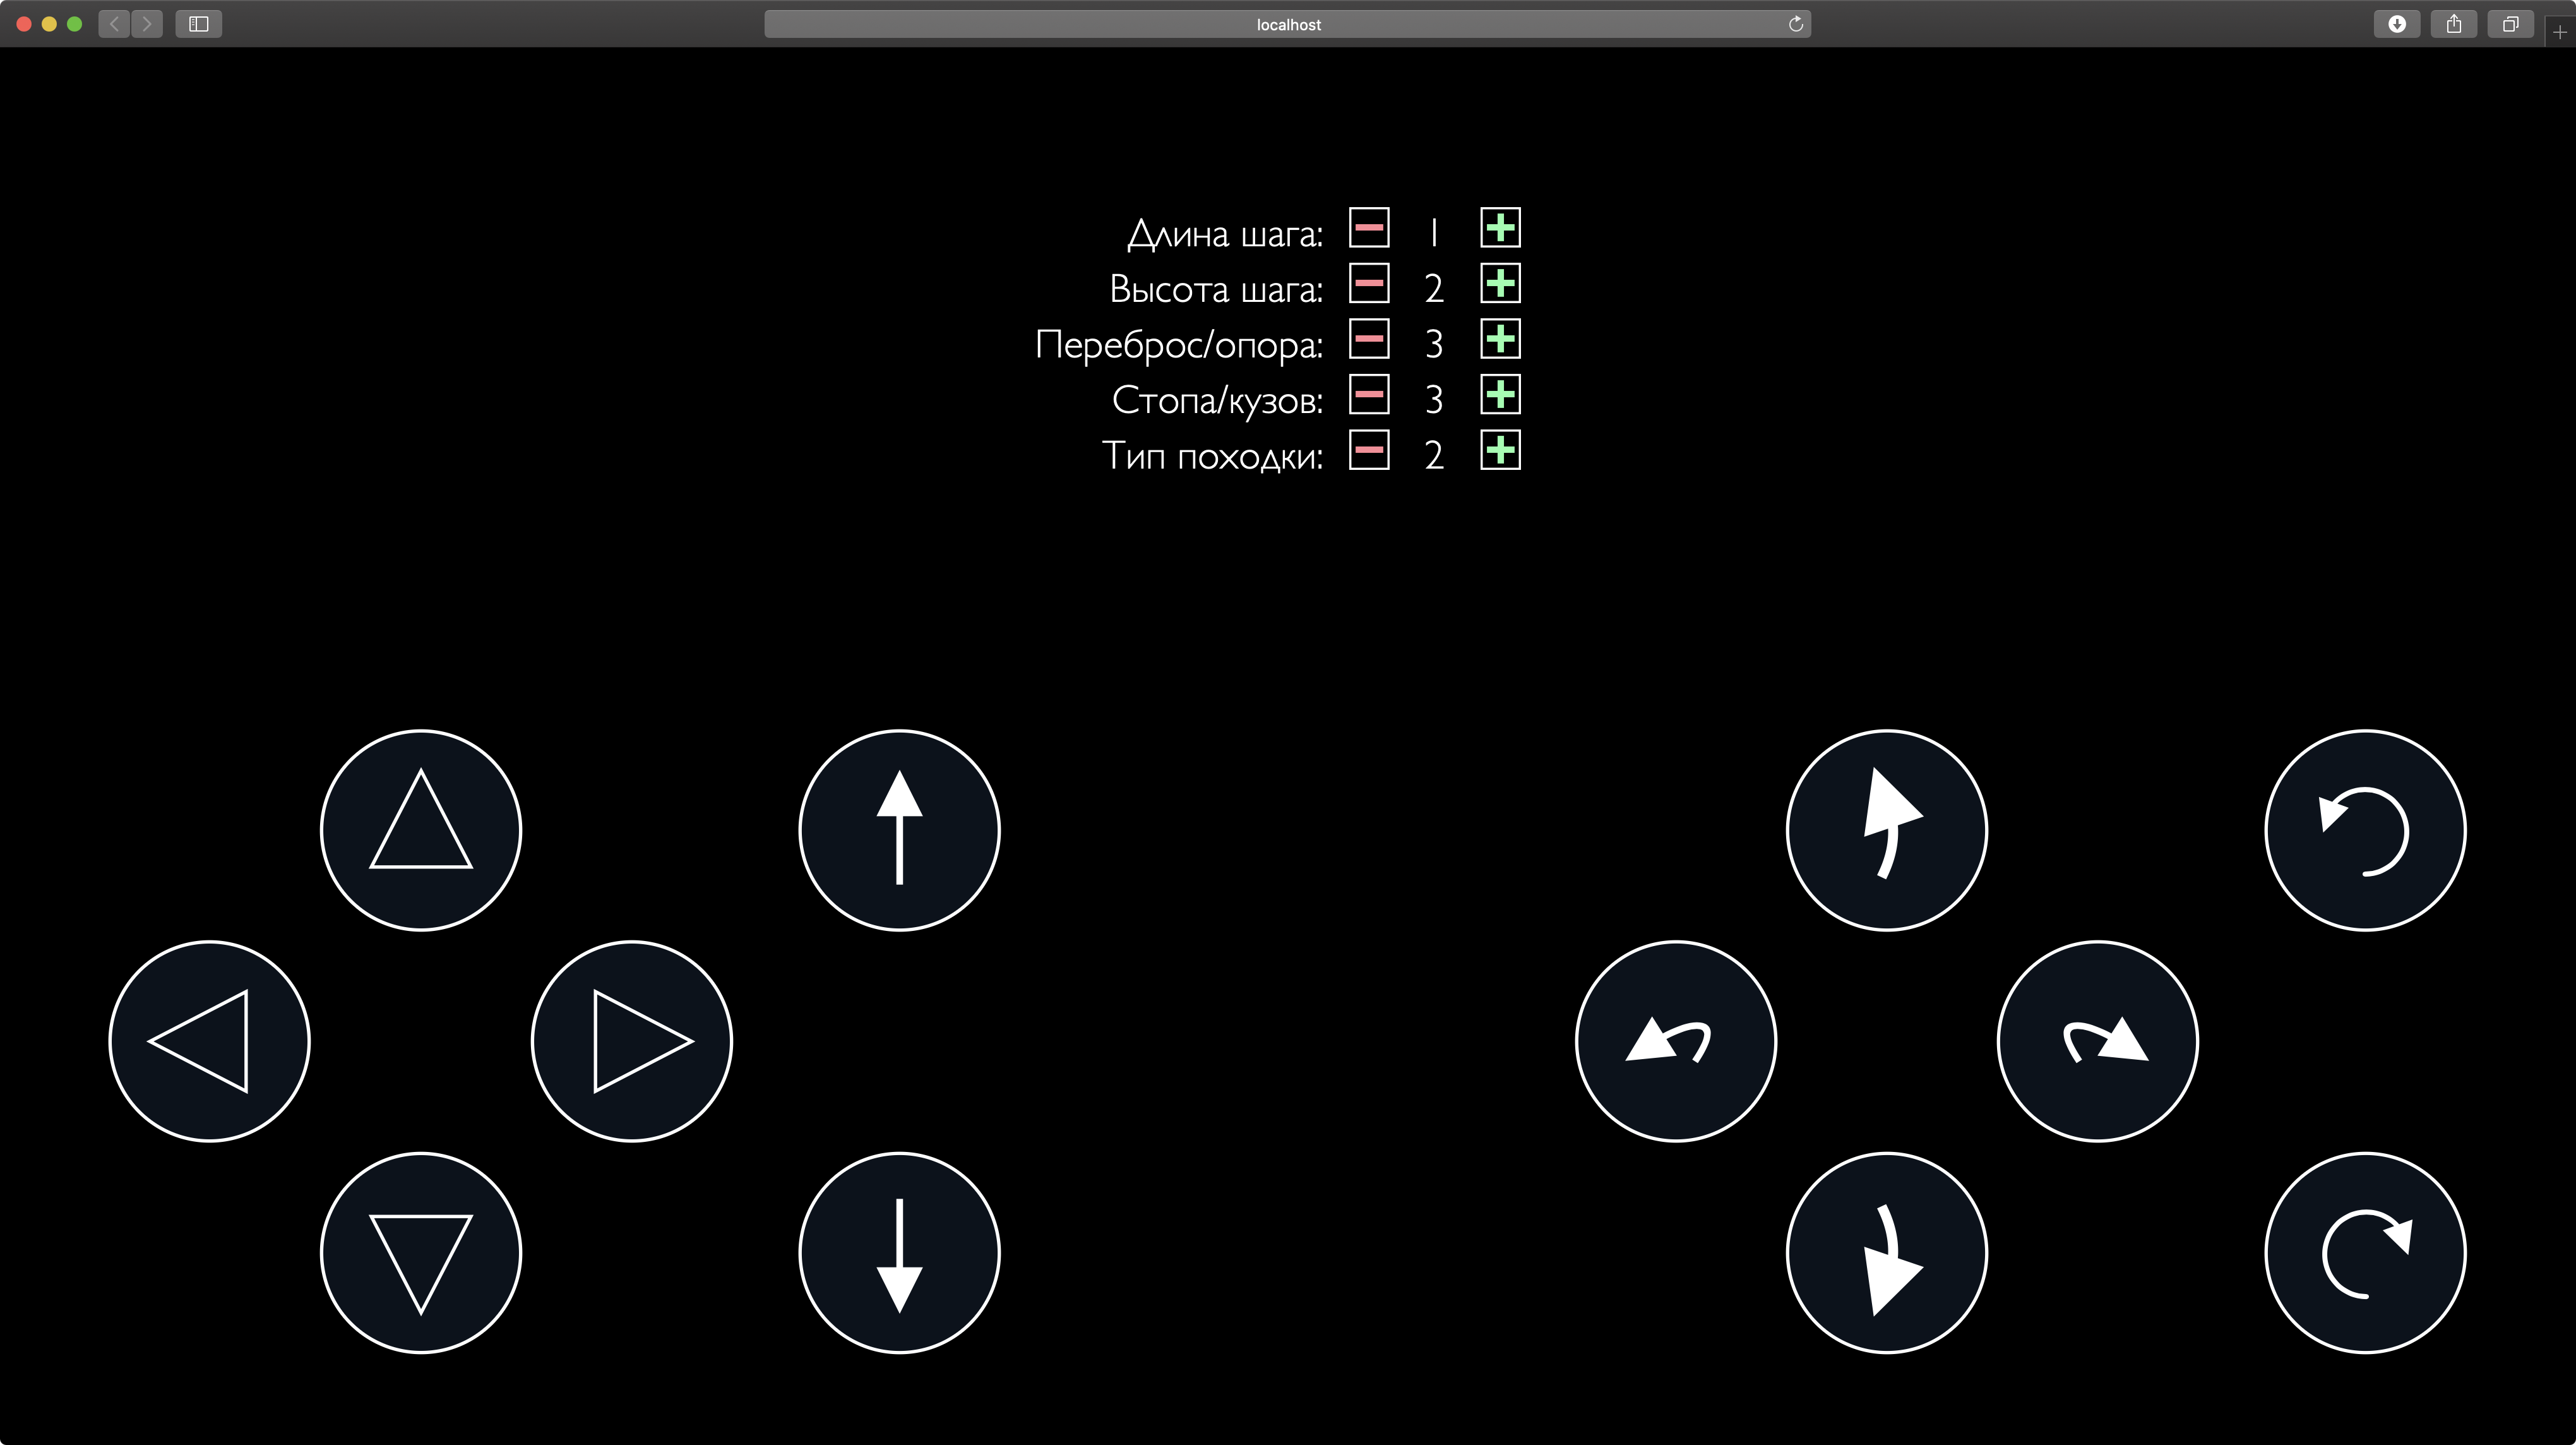
\includegraphics[width = \linewidth]{img/test1}
	\caption{Тестирование web интерфейса управления на компьютере}
	\label{img:test1}
\end{figure}

\begin{figure}[h!]
	\centering
	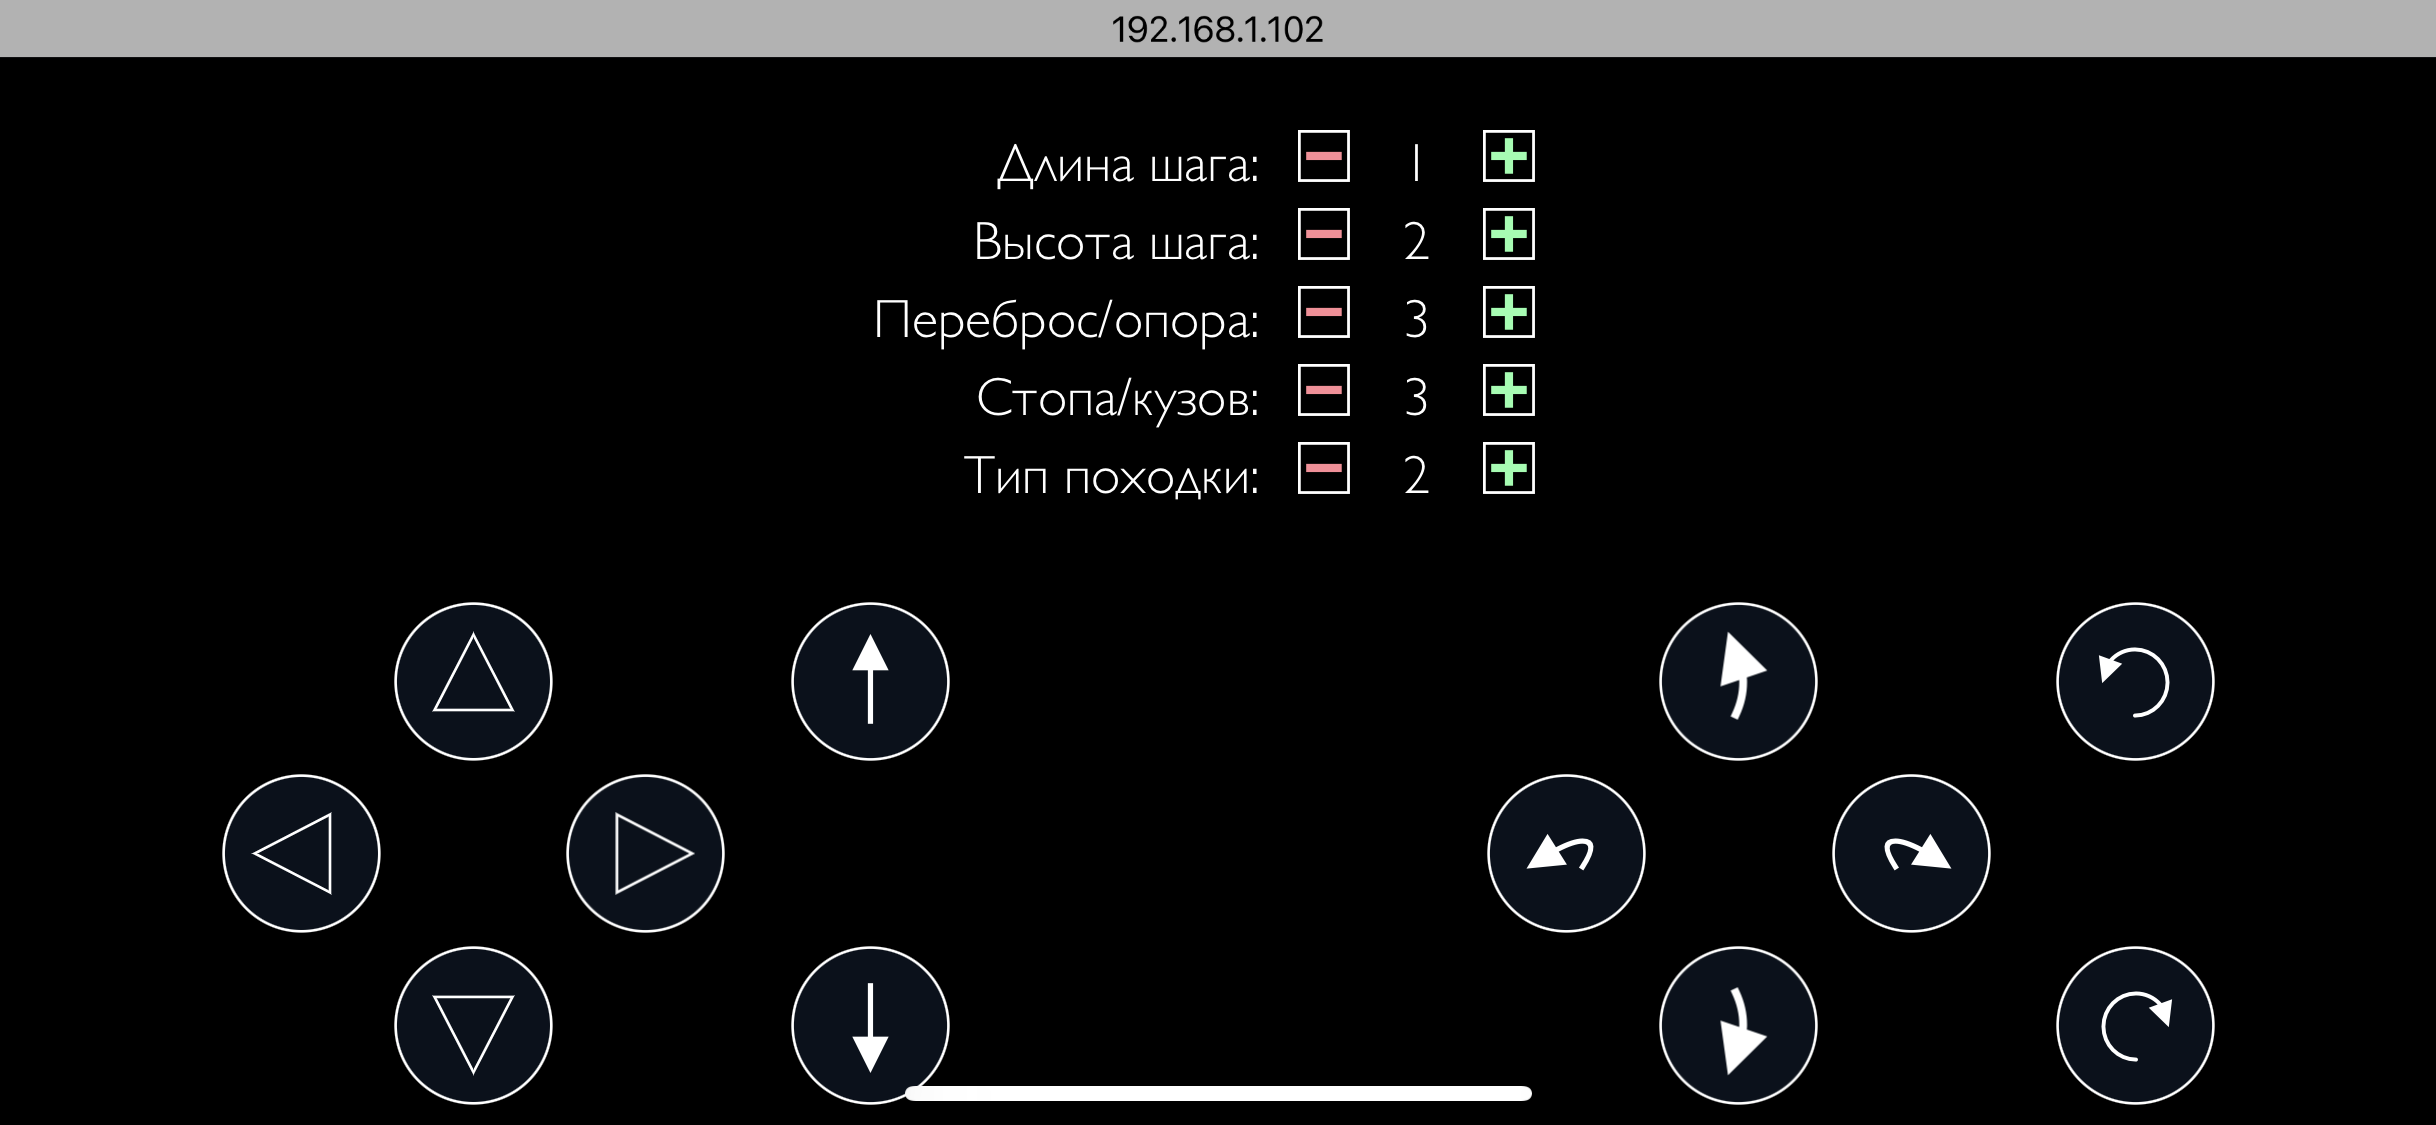
\includegraphics[width = \linewidth]{img/test2}
	\caption{Тестирование web интерфейса управления на смартфоне (горизонтальная ориентация)}
	\label{img:test2}
\end{figure}

\begin{figure}[h!]
	\centering
	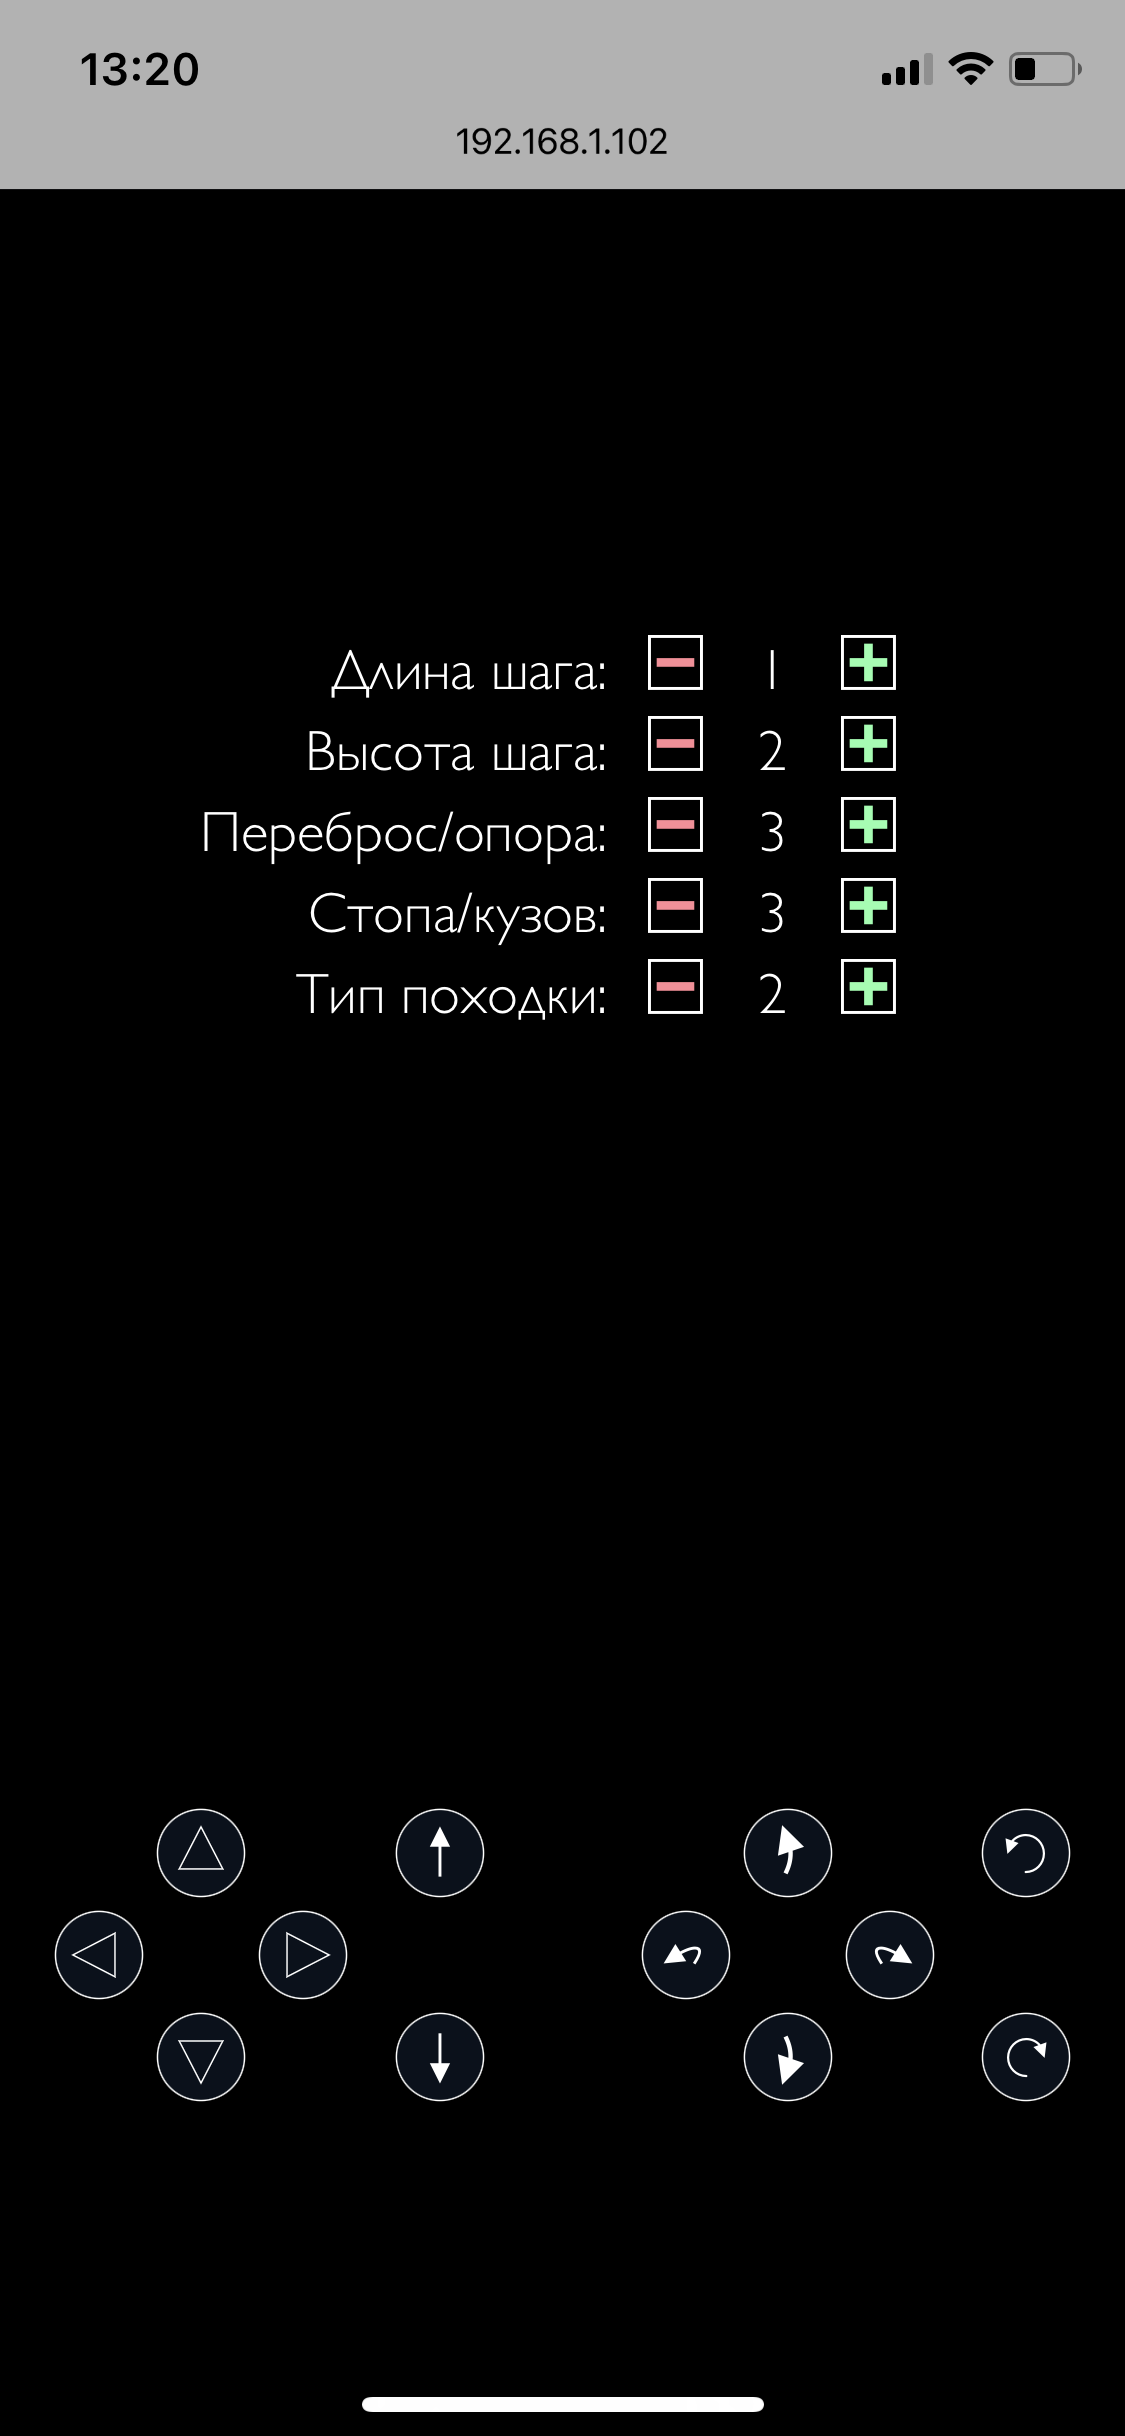
\includegraphics[height = 0.5\textheight]{img/test3}
	\caption{Тестирование web интерфейса управления на смартфоне (вертикальная ориентация)}
	\label{img:test3}
\end{figure}

Тестирование адаптивности и кросплатформенности при разработке web интерфейса управления проводилось в браузере Safari на Apple iMac 27 с разрешением экрана 5120 x 2880, а также на Apple iPhone X c разрешением экрана 2436×1125. Как можно увидеть на рисунках \ref{img:test1} – \ref{img:test3}, интерфейс успешно адаптируется к различному разрешению экрана, а также к ориентации экрана. Также из тестов видно, что синхронизация параметров между интерфейсами выполняется стабильно.

\begin{figure}[h!]
	\centering
	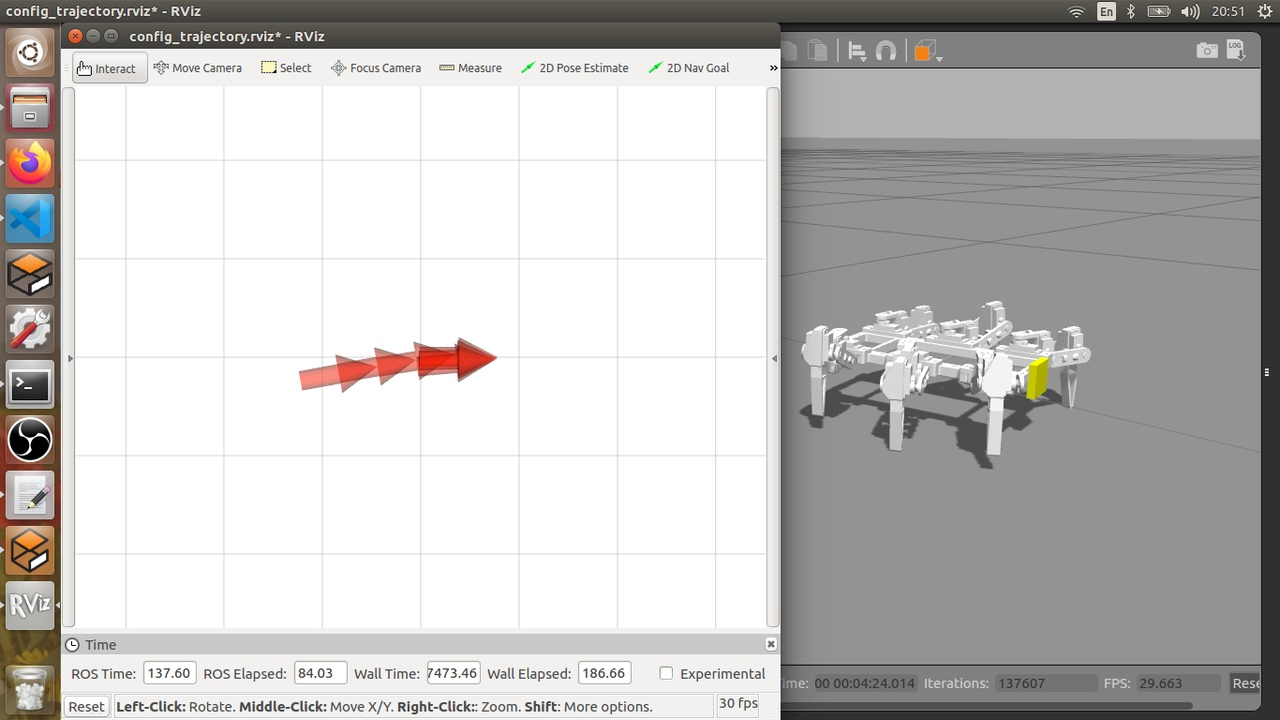
\includegraphics[width = \linewidth]{img/test4}
	\caption{Тест походки прямо}
	\label{img:test4}
\end{figure}

\begin{figure}[h!]
	\centering
	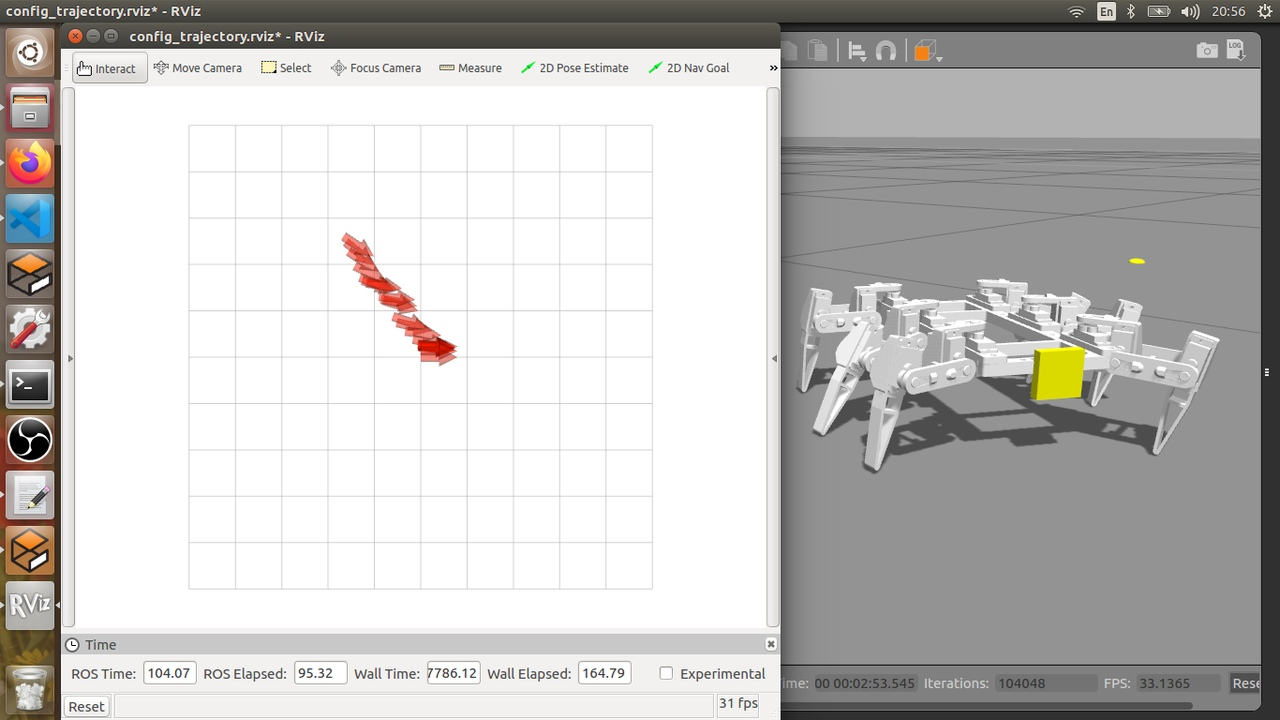
\includegraphics[width = \linewidth]{img/test5}
	\caption{Тест походки по диагонали}
	\label{img:test5}
\end{figure}

\begin{figure}[h!]
	\centering
	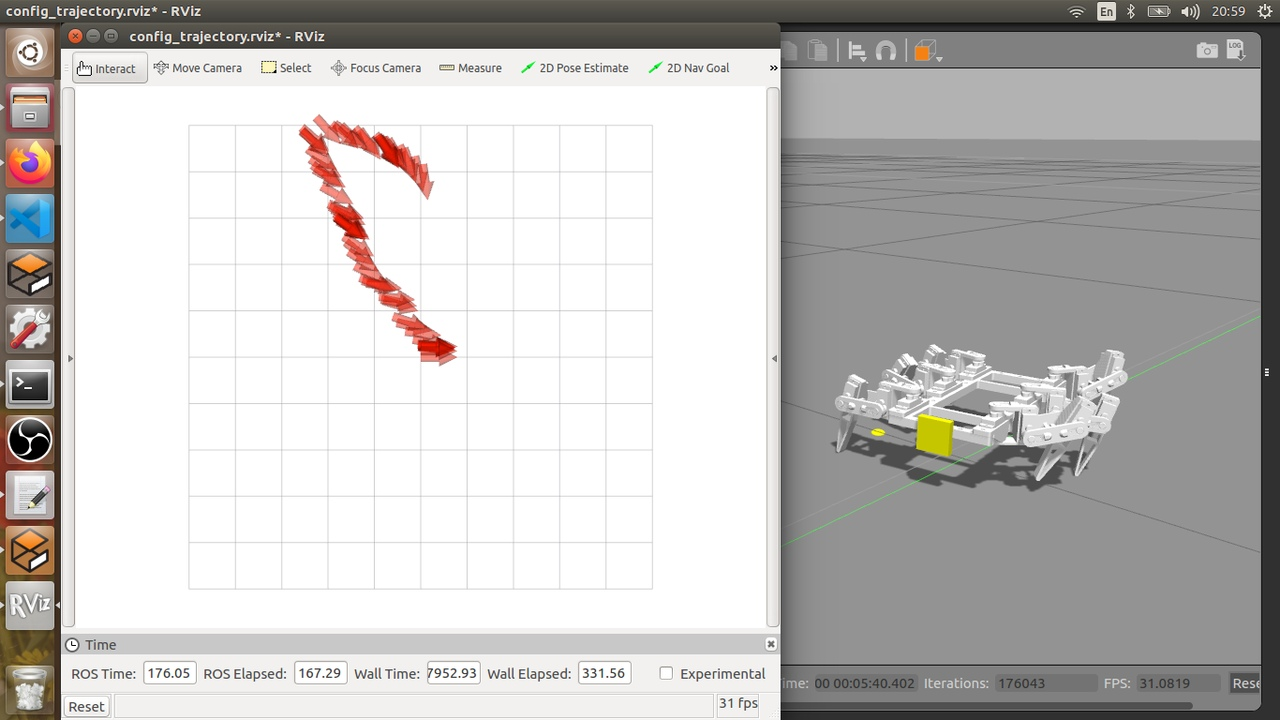
\includegraphics[width = \linewidth]{img/test6}
	\caption{Тест походки с разворотом}
	\label{img:test6}
\end{figure}

\begin{figure}[h!]
	\centering
	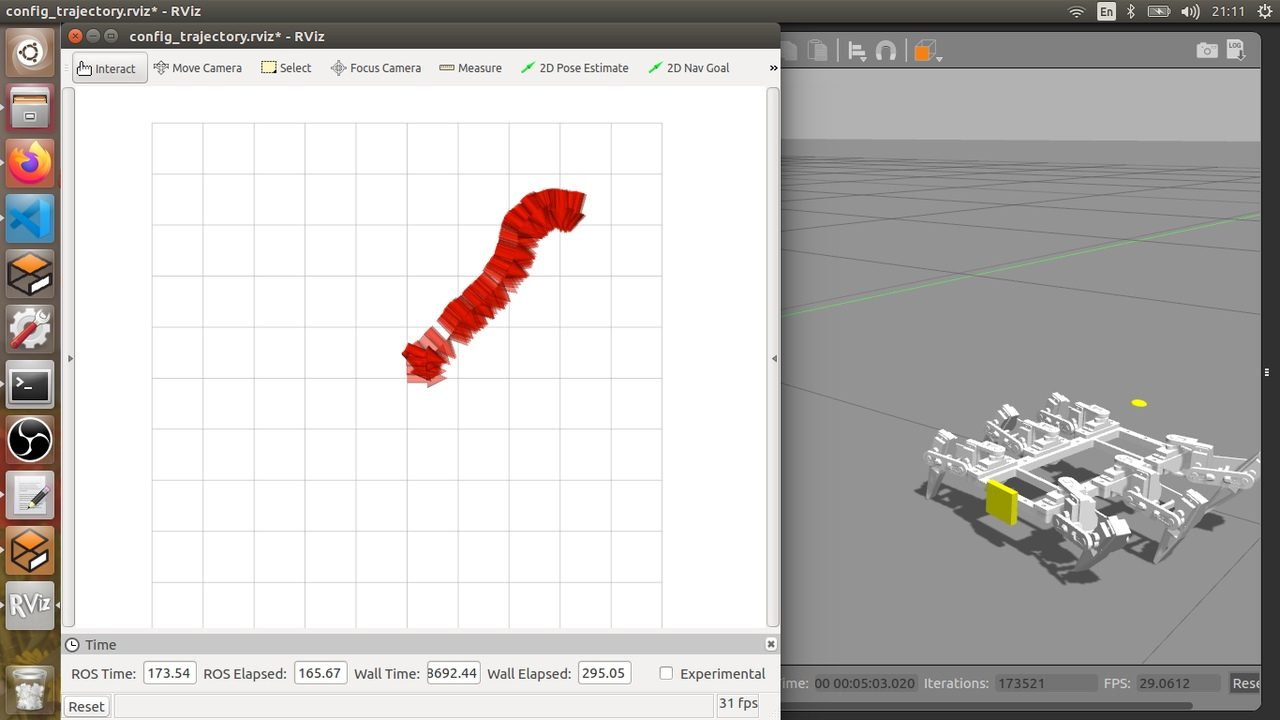
\includegraphics[width = \linewidth]{img/test7}
	\caption{Тест походки боком и поворота вокруг своей оси}
	\label{img:test7}
\end{figure}

\clearpage
\section {Выводы по главе}

В данной главе были проведены тесты разработанной системы управления роботом-гексаподом. Как можно видеть на рисунках \ref{img:test4} – \ref{img:test7} различные типы походок при управлении оператором выполняются успешно, есть небольшая погрешность, выражающаяся в незначительном отклонении от траектории, в виду неидеальности модели и различных факторов, влияющих на походку. Управление как с web интерфейса, так и с аппаратного джойстика работает стабильно, без перебоев. Условия адаптивности, кросплатформенности, а также синхронизации между экземплярами интерфейсов управления, согласно поставленной задачи, также успешно прошли все необходимые испытания.